\documentclass[tikz,border=10pt]{standalone}
\usepackage[T1]{fontenc}
\usepackage[scaled=0.95]{helvet}
\renewcommand{\familydefault}{\sfdefault}
\usepackage{xcolor}
\usetikzlibrary{arrows.meta,shapes.geometric,calc}

% ---------- palette ----------
\definecolor{gwnavy}{HTML}{1F3A5F}
\definecolor{gwteal}{HTML}{0F766E}
\definecolor{gwamber}{HTML}{B45309}
\definecolor{gwgreen}{HTML}{15803D}
\definecolor{gwslate}{HTML}{475569}
\definecolor{gwviolet}{HTML}{6D28D9}
\definecolor{gwblue}{HTML}{1D4ED8}

% ---------- step badge ----------
\newcommand{\sn}[1]{\tikz[baseline=(c.base)]\node[circle,fill=gwnavy,text=white,inner sep=0pt,minimum size=0.36cm,text width=0.36cm,align=center,font=\bfseries\scriptsize](c){#1};}

% ---------- styles ----------
\tikzset{
  box/.style={draw=#1!75!black, fill=#1!7, rounded corners=3pt, line width=0.8pt, align=left, font=\small},
  flow/.style={-{Stealth[length=2.6mm,width=2mm]}, line width=1.1pt, gwnavy},
  dbw/.style={-{Stealth[length=2.2mm,width=1.7mm]}, dashed, line width=0.8pt, gwslate},
  dbr/.style={{Stealth[length=2.2mm,width=1.7mm]}-, dashed, line width=0.8pt, gwslate},
  dbrw/.style={{Stealth[length=2.2mm,width=1.7mm]}-{Stealth[length=2.2mm,width=1.7mm]}, dashed, line width=0.8pt, gwslate},
  opt/.style={{Stealth[length=2.2mm,width=1.7mm]}-{Stealth[length=2.2mm,width=1.7mm]}, dashed, line width=0.9pt, gwviolet},
  lbl/.style={font=\scriptsize\bfseries, text=gwnavy, fill=white, inner sep=1.2pt},
  lbls/.style={font=\scriptsize, text=gwslate, inner sep=1pt},
}

% \blk{name}{color}{x1}{y1}{x2}{y2}{extra}{text}
\newcommand{\blk}[8]{%
  \pgfmathsetlengthmacro{\bw}{(#5-#3)*1cm}%
  \pgfmathsetlengthmacro{\bh}{(#6-#4)*1cm}%
  \pgfmathsetlengthmacro{\tw}{(#5-#3)*1cm-10pt}%
  \node[box=#2,#7,anchor=south west,minimum width=\bw,minimum height=\bh,text width=\tw,inner sep=5pt](#1) at (#3,#4){#8};}

% \cont{color}{x1}{y1}{x2}{y2}{title}
\newcommand{\cont}[6]{%
  \draw[draw=#1!70!black, fill=#1!4, rounded corners=5pt, line width=1pt] (#2,#3) rectangle (#4,#5);
  \node[anchor=north west, font=\small\bfseries, text=#1!60!black] at (#2+0.2,#5-0.12) {#6};}

\begin{document}
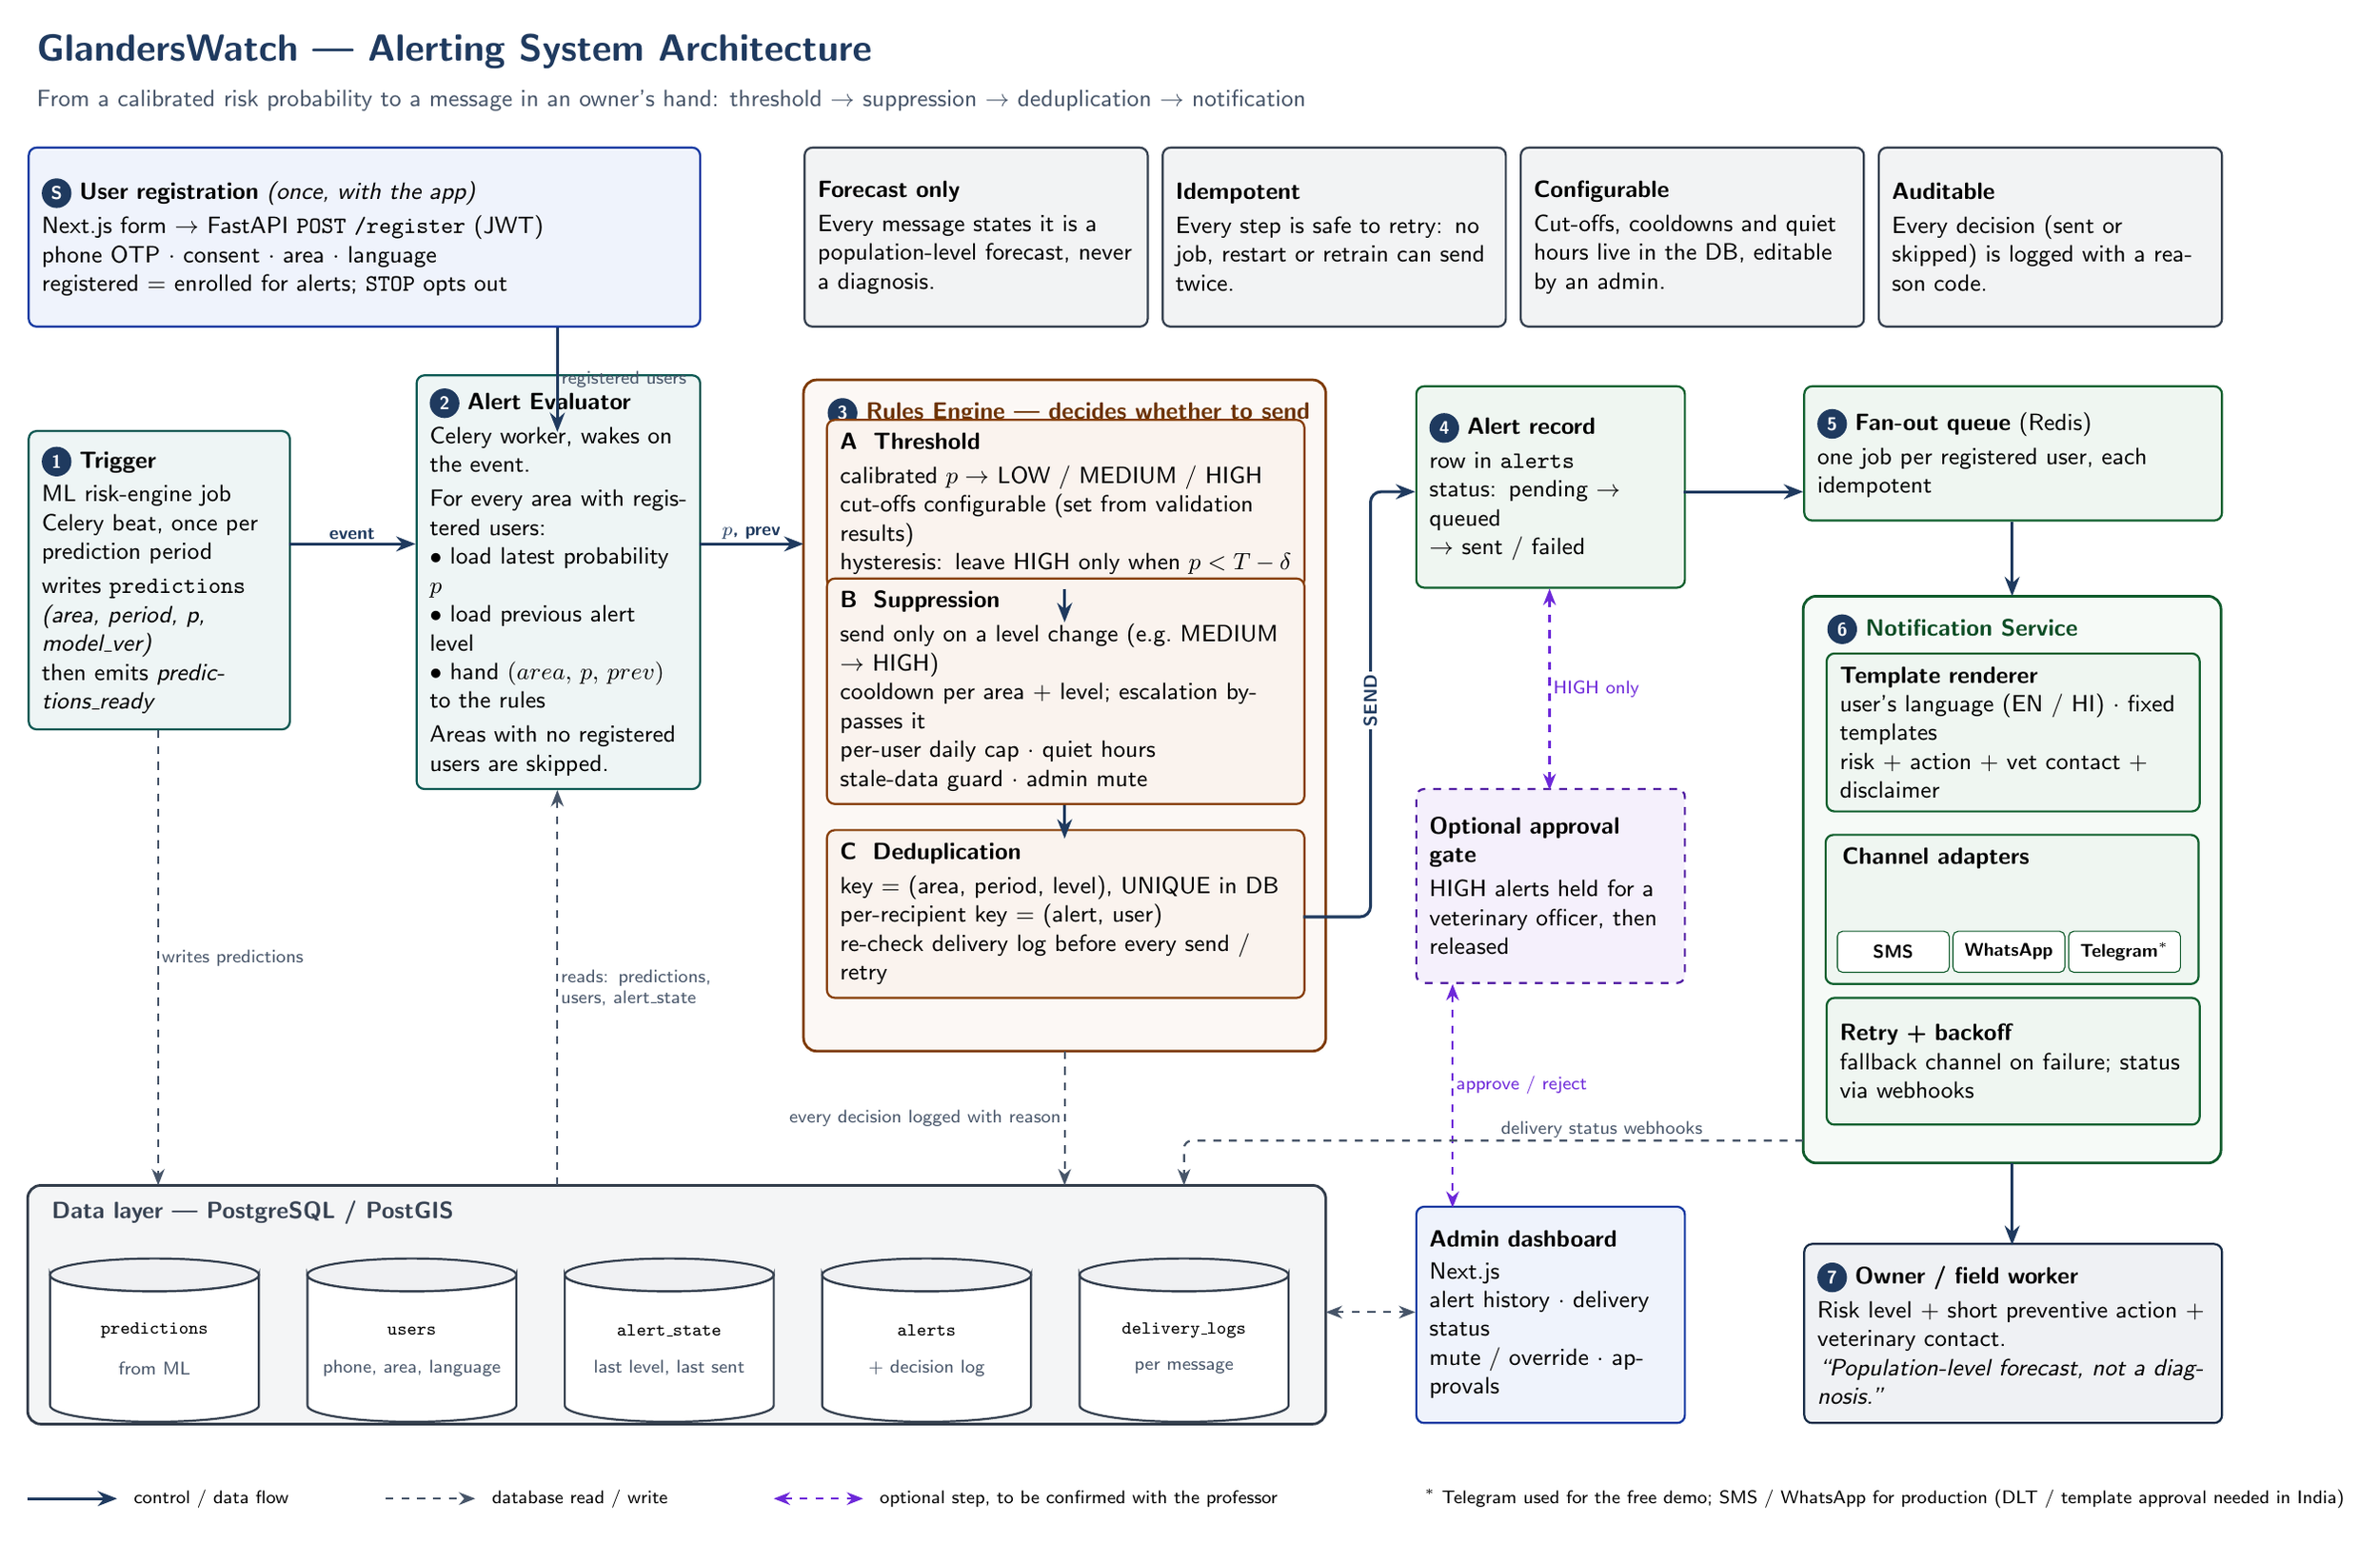
\begin{tikzpicture}[x=1cm,y=1cm]

% ================= TITLE =================
\node[anchor=west, font=\Large\bfseries, text=gwnavy] at (0.4,18.9) {GlandersWatch --- Alerting System Architecture};
\node[anchor=west, font=\small, text=gwslate] at (0.4,18.25) {From a calibrated risk probability to a message in an owner's hand: threshold $\rightarrow$ suppression $\rightarrow$ deduplication $\rightarrow$ notification};

% ================= TOP LANE =================

\blk{intake}{gwblue}{0.4}{15.2}{9.4}{17.6}{}{\textbf{\sn{S}\ User registration} \textit{(once, with the app)}\\[2pt]
Next.js form $\rightarrow$ FastAPI \texttt{POST /register} (JWT)\\
phone OTP $\cdot$ consent $\cdot$ area $\cdot$ language\\
registered = enrolled for alerts; \texttt{STOP} opts out}

\blk{p1}{gwslate}{10.8}{15.2}{15.4}{17.6}{}{\textbf{Forecast only}\\[2pt]Every message states it is a population-level forecast, never a diagnosis.}
\blk{p2}{gwslate}{15.6}{15.2}{20.2}{17.6}{}{\textbf{Idempotent}\\[2pt]Every step is safe to retry: no job, restart or retrain can send twice.}
\blk{p3}{gwslate}{20.4}{15.2}{25.0}{17.6}{}{\textbf{Configurable}\\[2pt]Cut-offs, cooldowns and quiet hours live in the DB, editable by an admin.}
\blk{p4}{gwslate}{25.2}{15.2}{29.8}{17.6}{}{\textbf{Auditable}\\[2pt]Every decision (sent or skipped) is logged with a reason code.}

% ================= MAIN BAND =================
\blk{trig}{gwteal}{0.4}{9.8}{3.9}{13.8}{}{\textbf{\sn{1}\ Trigger}\\[2pt]
ML risk-engine job\\
Celery beat, once per prediction period\\[2pt]
writes \texttt{predictions}\\
\textit{(area, period, p, model\_ver)}\\
then emits \textit{predictions\_ready}}

\blk{eval}{gwteal}{5.6}{9.0}{9.4}{13.8}{}{\textbf{\sn{2}\ Alert Evaluator}\\[2pt]
Celery worker, wakes on the event.\\[2pt]
For every area with registered users:\\
$\bullet$ load latest probability $p$\\
$\bullet$ load previous alert level\\
$\bullet$ hand $(area,\,p,\,prev)$ to the rules\\[2pt]
Areas with no registered users are skipped.}

% ---- rules engine ----
\cont{gwamber}{10.8}{5.5}{17.8}{14.5}{\sn{3}\ Rules Engine --- decides whether to send}
\blk{rA}{gwamber}{11.1}{11.7}{17.5}{13.8}{}{\textbf{A\ \ Threshold}\\[2pt]
calibrated $p \rightarrow$ LOW / MEDIUM / HIGH\\
cut-offs configurable (set from validation results)\\
hysteresis: leave HIGH only when $p < T-\delta$}
\blk{rB}{gwamber}{11.1}{8.8}{17.5}{11.25}{}{\textbf{B\ \ Suppression}\\[2pt]
send only on a level change (e.g.\ MEDIUM $\rightarrow$ HIGH)\\
cooldown per area + level; escalation bypasses it\\
per-user daily cap $\cdot$ quiet hours\\
stale-data guard $\cdot$ admin mute}
\blk{rC}{gwamber}{11.1}{6.2}{17.5}{8.35}{}{\textbf{C\ \ Deduplication}\\[2pt]
key = (area, period, level), UNIQUE in DB\\
per-recipient key = (alert, user)\\
re-check delivery log before every send / retry}
\draw[flow] (14.3,11.7) -- (14.3,11.25);
\draw[flow] (14.3,8.8) -- (14.3,8.35);

% ---- alert record + optional gate ----
\blk{rec}{gwgreen}{19.0}{11.7}{22.6}{14.4}{}{\textbf{\sn{4}\ Alert record}\\[2pt]
row in \texttt{alerts}\\
status: pending $\rightarrow$ queued\\
$\rightarrow$ sent / failed}
\blk{gate}{gwviolet}{19.0}{6.4}{22.6}{9.0}{dashed}{\textbf{Optional approval gate}\\[2pt]
HIGH alerts held for a veterinary officer, then released}

% ---- right column ----
\blk{que}{gwgreen}{24.2}{12.6}{29.8}{14.4}{}{\textbf{\sn{5}\ Fan-out queue} (Redis)\\[2pt]
one job per registered user, each idempotent}

\cont{gwgreen}{24.2}{4.0}{29.8}{11.6}{\sn{6}\ Notification Service}
\blk{ren}{gwgreen}{24.5}{8.7}{29.5}{10.5}{}{\textbf{Template renderer}\\
user's language (EN / HI) $\cdot$ fixed templates\\
risk + action + vet contact + disclaimer}
\draw[box=gwgreen, rounded corners=3pt, line width=0.8pt] (24.5,6.4) rectangle (29.5,8.4);
\node[anchor=north west, font=\small\bfseries, text=black] at (24.6,8.35) {Channel adapters};
\foreach \x/\t in {24.65/SMS,26.2/WhatsApp,27.75/Telegram$^{*}$}{
  \node[draw=gwgreen!70!black, fill=white, rounded corners=2pt, font=\scriptsize\bfseries, minimum width=1.5cm, minimum height=0.55cm, anchor=south west, inner sep=1pt] at (\x,6.55) {\t};}
\blk{ret}{gwgreen}{24.5}{4.5}{29.5}{6.2}{}{\textbf{Retry + backoff}\\
fallback channel on failure; status via \mbox{webhooks}}

\blk{rcp}{gwnavy}{24.2}{0.5}{29.8}{2.9}{}{\textbf{\sn{7}\ Owner / field worker}\\[2pt]
Risk level + short preventive action + veterinary contact.\\
\textit{``Population-level forecast, not a diagnosis.''}}

% ================= DATA LAYER =================
\draw[draw=gwslate!70!black, fill=gwslate!6, rounded corners=5pt, line width=1pt] (0.4,0.5) rectangle (17.8,3.7);
\node[anchor=north west, font=\small\bfseries, text=gwslate!80!black] at (0.6,3.62) {Data layer --- PostgreSQL / PostGIS};
\foreach \c/\n/\d in {2.1/predictions/{from ML},5.55/users/{phone, area, language},9.0/alert\_state/{last level, last sent},12.45/alerts/{+ decision log},15.9/delivery\_logs/{per message}}{
  \draw[draw=gwslate!75!black, fill=white, line width=0.8pt] (\c-1.4,0.75) -- (\c-1.4,2.5) arc (180:360:1.4 and 0.22) -- (\c+1.4,0.75) arc (360:180:1.4 and 0.22);
  \draw[draw=gwslate!75!black, fill=gwslate!8, line width=0.8pt] (\c,2.5) ellipse (1.4 and 0.22);
  \node[font=\scriptsize\bfseries\ttfamily, text=black] at (\c,1.75) {\n};
  \node[font=\scriptsize, text=gwslate] at (\c,1.25) {\d};
}

\blk{adm}{gwblue}{19.0}{0.5}{22.6}{3.4}{}{\textbf{Admin dashboard}\\[1pt]
Next.js\\
alert history $\cdot$ delivery status\\
mute / override $\cdot$ approvals}

% ================= ARROWS =================
% setup path
\draw[flow] (7.5,15.2) -- (7.5,13.8) node[midway,right,lbls]{registered users};
% trigger -> evaluator -> rules
\draw[flow] (3.9,12.3) -- (5.6,12.3) node[midway,above,lbl]{event};
\draw[flow] (9.4,12.3) -- (10.8,12.3) node[midway,above,lbl]{$p$, prev};
% SEND path
\draw[flow, rounded corners=4pt] (17.5,7.3) -- (18.4,7.3) -- (18.4,13.0) -- (19.0,13.0);
\node[lbl, rotate=90] at (18.4,10.2) {SEND};
% record -> queue -> service -> recipient
\draw[flow] (22.6,13.0) -- (24.2,13.0);
\draw[flow] (27.0,12.6) -- (27.0,11.6);
\draw[flow] (27.0,4.0) -- (27.0,2.9);
% optional gate
\draw[opt] (20.8,11.7) -- (20.8,9.0) node[midway,right,lbls,text=gwviolet]{HIGH only};
\draw[opt] (19.5,6.4) -- (19.5,3.4) node[pos=0.45,right,lbls,text=gwviolet]{approve / reject};
% database arrows
\draw[dbw] (2.15,9.8) -- (2.15,3.7) node[midway,right,lbls]{writes predictions};
\draw[dbr] (7.5,9.0) -- (7.5,3.7) node[pos=0.5,right,lbls,text width=2.6cm,align=left]{reads: predictions, users, alert\_state};
\draw[dbw] (14.3,5.5) -- (14.3,3.7) node[midway,left,lbls]{every decision logged with reason};
\draw[dbw, rounded corners=3pt] (24.2,4.3) -- (15.9,4.3) -- (15.9,3.7);
\node[lbls, anchor=south] at (21.5,4.3) {delivery status webhooks};
\draw[dbrw] (17.8,2.0) -- (19.0,2.0);

% ================= LEGEND =================
\draw[flow] (0.4,-0.5) -- (1.6,-0.5);
\node[anchor=west, font=\scriptsize] at (1.7,-0.5) {control / data flow};
\draw[dbw] (5.2,-0.5) -- (6.4,-0.5);
\node[anchor=west, font=\scriptsize] at (6.5,-0.5) {database read / write};
\draw[opt] (10.4,-0.5) -- (11.6,-0.5);
\node[anchor=west, font=\scriptsize] at (11.7,-0.5) {optional step, to be confirmed with the professor};
\node[anchor=west, font=\scriptsize] at (19.0,-0.5) {$^{*}$ Telegram used for the free demo; SMS / WhatsApp for production (DLT / template approval needed in India)};

\end{tikzpicture}
\end{document}

% \documentclass[tikz,border=10pt]{standalone}
% \usepackage[T1]{fontenc}
% \usepackage[scaled=0.95]{helvet}
% \renewcommand{\familydefault}{\sfdefault}
% \usepackage{xcolor}
% \usetikzlibrary{arrows.meta,shapes.geometric,calc}

% % ---------- palette ----------
% \definecolor{gwnavy}{HTML}{1F3A5F}
% \definecolor{gwteal}{HTML}{0F766E}
% \definecolor{gwamber}{HTML}{B45309}
% \definecolor{gwgreen}{HTML}{15803D}
% \definecolor{gwslate}{HTML}{475569}
% \definecolor{gwviolet}{HTML}{6D28D9}
% \definecolor{gwblue}{HTML}{1D4ED8}

% % ---------- step badge ----------
% \newcommand{\sn}[1]{\tikz[baseline=(c.base)]\node[circle,fill=gwnavy,text=white,inner sep=0pt,minimum size=0.36cm,text width=0.36cm,align=center,font=\bfseries\tiny](c){#1};}

% % ---------- styles ----------
% \tikzset{
%   box/.style={draw=#1!75!black, fill=#1!7, rounded corners=3pt, line width=0.8pt, align=left, font=\scriptsize},
%   flow/.style={-{Stealth[length=2.6mm,width=2mm]}, line width=1.1pt, gwnavy},
%   dbw/.style={-{Stealth[length=2.2mm,width=1.7mm]}, dashed, line width=0.8pt, gwslate},
%   dbr/.style={{Stealth[length=2.2mm,width=1.7mm]}-, dashed, line width=0.8pt, gwslate},
%   dbrw/.style={{Stealth[length=2.2mm,width=1.7mm]}-{Stealth[length=2.2mm,width=1.7mm]}, dashed, line width=0.8pt, gwslate},
%   opt/.style={{Stealth[length=2.2mm,width=1.7mm]}-{Stealth[length=2.2mm,width=1.7mm]}, dashed, line width=0.9pt, gwviolet},
%   lbl/.style={font=\tiny\bfseries, text=gwnavy, fill=white, inner sep=1.2pt},
%   lbls/.style={font=\tiny, text=gwslate, inner sep=1pt},
% }

% % \blk{name}{color}{x1}{y1}{x2}{y2}{extra}{text}
% \newcommand{\blk}[8]{%
%   \pgfmathsetlengthmacro{\bw}{(#5-#3)*1cm}%
%   \pgfmathsetlengthmacro{\bh}{(#6-#4)*1cm}%
%   \pgfmathsetlengthmacro{\tw}{(#5-#3)*1cm-10pt}%
%   \node[box=#2,#7,anchor=south west,minimum width=\bw,minimum height=\bh,text width=\tw,inner sep=5pt](#1) at (#3,#4){#8};}

% % \cont{color}{x1}{y1}{x2}{y2}{title}
% \newcommand{\cont}[6]{%
%   \draw[draw=#1!70!black, fill=#1!4, rounded corners=5pt, line width=1pt] (#2,#3) rectangle (#4,#5);
%   \node[anchor=north west, font=\small\bfseries, text=#1!60!black] at (#2+0.2,#5-0.12) {#6};}

% \begin{document}
% \begin{tikzpicture}[x=1cm,y=1cm]

% % ================= TITLE =================
% \node[anchor=west, font=\Large\bfseries, text=gwnavy] at (0.4,18.9) {GlandersWatch --- Alerting System Architecture};
% \node[anchor=west, font=\small, text=gwslate] at (0.4,18.25) {From a calibrated risk probability to a message in an owner's hand: threshold $\rightarrow$ suppression $\rightarrow$ deduplication $\rightarrow$ notification};

% % ================= TOP LANE =================

% \blk{intake}{gwblue}{0.4}{15.2}{9.4}{17.6}{}{\textbf{\sn{S}\ User registration} \textit{(once, with the app)}\\[2pt]
% Next.js form $\rightarrow$ FastAPI \texttt{POST /register} (JWT)\\
% phone OTP $\cdot$ consent $\cdot$ area $\cdot$ language\\
% registered = enrolled for alerts; \texttt{STOP} opts out}

% \blk{p1}{gwslate}{10.8}{15.2}{15.4}{17.6}{}{\textbf{Forecast only}\\[2pt]Every message states it is a population-level forecast, never a diagnosis.}
% \blk{p2}{gwslate}{15.6}{15.2}{20.2}{17.6}{}{\textbf{Idempotent}\\[2pt]Every step is safe to retry: no job, restart or retrain can send twice.}
% \blk{p3}{gwslate}{20.4}{15.2}{25.0}{17.6}{}{\textbf{Configurable}\\[2pt]Cut-offs, cooldowns and quiet hours live in the DB, editable by an admin.}
% \blk{p4}{gwslate}{25.2}{15.2}{29.8}{17.6}{}{\textbf{Auditable}\\[2pt]Every decision (sent or skipped) is logged with a reason code.}

% % ================= MAIN BAND =================
% \blk{trig}{gwteal}{0.4}{9.8}{3.9}{13.8}{}{\textbf{\sn{1}\ Trigger}\\[2pt]
% ML risk-engine job\\
% Celery beat, once per prediction period\\[2pt]
% writes \texttt{predictions}\\
% \textit{(area, period, p, model\_ver)}\\
% then emits \textit{predictions\_ready}}

% \blk{eval}{gwteal}{5.6}{9.0}{9.4}{13.8}{}{\textbf{\sn{2}\ Alert Evaluator}\\[2pt]
% Celery worker, wakes on the event.\\[2pt]
% For every area with registered users:\\
% $\bullet$ load latest probability $p$\\
% $\bullet$ load previous alert level\\
% $\bullet$ hand $(area,\,p,\,prev)$ to the rules\\[2pt]
% Areas with no registered users are skipped.}

% % ---- rules engine ----
% \cont{gwamber}{10.8}{5.5}{17.8}{14.5}{\sn{3}\ Rules Engine --- decides whether to send}
% \blk{rA}{gwamber}{11.1}{11.7}{17.5}{13.8}{}{\textbf{A\ \ Threshold}\\[2pt]
% calibrated $p \rightarrow$ LOW / MEDIUM / HIGH\\
% cut-offs configurable (set from validation results)\\
% hysteresis: leave HIGH only when $p < T-\delta$}
% \blk{rB}{gwamber}{11.1}{8.8}{17.5}{11.25}{}{\textbf{B\ \ Suppression}\\[2pt]
% send only on a level change (e.g.\ MEDIUM $\rightarrow$ HIGH)\\
% cooldown per area + level; escalation bypasses it\\
% per-user daily cap $\cdot$ quiet hours\\
% stale-data guard $\cdot$ admin mute}
% \blk{rC}{gwamber}{11.1}{6.2}{17.5}{8.35}{}{\textbf{C\ \ Deduplication}\\[2pt]
% key = (area, period, level), UNIQUE in DB\\
% per-recipient key = (alert, user)\\
% re-check delivery log before every send / retry}
% \draw[flow] (14.3,11.7) -- (14.3,11.25);
% \draw[flow] (14.3,8.8) -- (14.3,8.35);

% % ---- alert record + optional gate ----
% \blk{rec}{gwgreen}{19.0}{11.7}{22.6}{14.4}{}{\textbf{\sn{4}\ Alert record}\\[2pt]
% row in \texttt{alerts}\\
% status: pending $\rightarrow$ queued\\
% $\rightarrow$ sent / failed}
% \blk{gate}{gwviolet}{19.0}{6.4}{22.6}{9.0}{dashed}{\textbf{Optional approval gate}\\[2pt]
% HIGH alerts held for a veterinary officer, then released}

% % ---- right column ----
% \blk{que}{gwgreen}{24.2}{12.6}{29.8}{14.4}{}{\textbf{\sn{5}\ Fan-out queue} (Redis)\\[2pt]
% one job per registered user, each idempotent}

% \cont{gwgreen}{24.2}{4.0}{29.8}{11.6}{\sn{6}\ Notification Service}
% \blk{ren}{gwgreen}{24.5}{8.7}{29.5}{10.5}{}{\textbf{Template renderer}\\
% user's language (EN / HI) $\cdot$ fixed templates\\
% risk + action + vet contact + disclaimer}
% \draw[box=gwgreen, rounded corners=3pt, line width=0.8pt] (24.5,6.4) rectangle (29.5,8.4);
% \node[anchor=north west, font=\scriptsize\bfseries, text=black] at (24.6,8.35) {Channel adapters};
% \foreach \x/\t in {24.65/SMS,26.2/WhatsApp,27.75/Telegram$^{*}$}{
%   \node[draw=gwgreen!70!black, fill=white, rounded corners=2pt, font=\tiny\bfseries, minimum width=1.5cm, minimum height=0.55cm, anchor=south west, inner sep=1pt] at (\x,6.55) {\t};}
% \blk{ret}{gwgreen}{24.5}{4.5}{29.5}{6.2}{}{\textbf{Retry + backoff}\\
% fallback channel on failure; status via \mbox{webhooks}}

% \blk{rcp}{gwnavy}{24.2}{0.5}{29.8}{2.9}{}{\textbf{\sn{7}\ Owner / field worker}\\[2pt]
% Risk level + short preventive action + veterinary contact.\\
% \textit{``Population-level forecast, not a diagnosis.''}}

% % ================= DATA LAYER =================
% \draw[draw=gwslate!70!black, fill=gwslate!6, rounded corners=5pt, line width=1pt] (0.4,0.5) rectangle (17.8,3.7);
% \node[anchor=north west, font=\small\bfseries, text=gwslate!80!black] at (0.6,3.62) {Data layer --- PostgreSQL / PostGIS};
% \foreach \c/\n/\d in {2.1/predictions/{from ML},5.55/users/{phone, area, language},9.0/alert\_state/{last level, last sent},12.45/alerts/{+ decision log},15.9/delivery\_logs/{per message}}{
%   \draw[draw=gwslate!75!black, fill=white, line width=0.8pt] (\c-1.4,0.75) -- (\c-1.4,2.5) arc (180:360:1.4 and 0.22) -- (\c+1.4,0.75) arc (360:180:1.4 and 0.22);
%   \draw[draw=gwslate!75!black, fill=gwslate!8, line width=0.8pt] (\c,2.5) ellipse (1.4 and 0.22);
%   \node[font=\scriptsize\bfseries\ttfamily, text=black] at (\c,1.75) {\n};
%   \node[font=\tiny, text=gwslate] at (\c,1.25) {\d};
% }

% \blk{adm}{gwblue}{19.0}{0.5}{22.6}{3.4}{}{\textbf{Admin dashboard}\\[1pt]
% Next.js\\
% alert history $\cdot$ delivery status\\
% mute / override $\cdot$ approvals}

% % ================= ARROWS =================
% % setup path
% \draw[flow] (7.5,15.2) -- (7.5,13.8) node[midway,right,lbls]{registered users};
% % trigger -> evaluator -> rules
% \draw[flow] (3.9,12.3) -- (5.6,12.3) node[midway,above,lbl]{event};
% \draw[flow] (9.4,12.3) -- (10.8,12.3) node[midway,above,lbl]{$p$, prev};
% % SEND path
% \draw[flow, rounded corners=4pt] (17.5,7.3) -- (18.4,7.3) -- (18.4,13.0) -- (19.0,13.0);
% \node[lbl, rotate=90] at (18.4,10.2) {SEND};
% % record -> queue -> service -> recipient
% \draw[flow] (22.6,13.0) -- (24.2,13.0);
% \draw[flow] (27.0,12.6) -- (27.0,11.6);
% \draw[flow] (27.0,4.0) -- (27.0,2.9);
% % optional gate
% \draw[opt] (20.8,11.7) -- (20.8,9.0) node[midway,right,lbls,text=gwviolet]{HIGH only};
% \draw[opt] (19.5,6.4) -- (19.5,3.4) node[pos=0.45,right,lbls,text=gwviolet]{approve / reject};
% % database arrows
% \draw[dbw] (2.15,9.8) -- (2.15,3.7) node[midway,right,lbls]{writes predictions};
% \draw[dbr] (7.5,9.0) -- (7.5,3.7) node[pos=0.5,right,lbls,text width=2.6cm,align=left]{reads: predictions, users, alert\_state};
% \draw[dbw] (14.3,5.5) -- (14.3,3.7) node[midway,left,lbls]{every decision logged with reason};
% \draw[dbw, rounded corners=3pt] (24.2,4.3) -- (15.9,4.3) -- (15.9,3.7);
% \node[lbls, anchor=south] at (21.5,4.3) {delivery status webhooks};
% \draw[dbrw] (17.8,2.0) -- (19.0,2.0);

% % ================= LEGEND =================
% \draw[flow] (0.4,-0.5) -- (1.6,-0.5);
% \node[anchor=west, font=\tiny] at (1.7,-0.5) {control / data flow};
% \draw[dbw] (5.2,-0.5) -- (6.4,-0.5);
% \node[anchor=west, font=\tiny] at (6.5,-0.5) {database read / write};
% \draw[opt] (10.4,-0.5) -- (11.6,-0.5);
% \node[anchor=west, font=\tiny] at (11.7,-0.5) {optional step, to be confirmed with the professor};
% \node[anchor=west, font=\tiny] at (19.0,-0.5) {$^{*}$ Telegram used for the free demo; SMS / WhatsApp for production (DLT / template approval needed in India)};

% \end{tikzpicture}
% \end{document}
